% Options for packages loaded elsewhere
\PassOptionsToPackage{unicode}{hyperref}
\PassOptionsToPackage{hyphens}{url}
%
\documentclass[
]{article}
\usepackage{lmodern}
\usepackage{amssymb,amsmath}
\usepackage{ifxetex,ifluatex}
\ifnum 0\ifxetex 1\fi\ifluatex 1\fi=0 % if pdftex
  \usepackage[T1]{fontenc}
  \usepackage[utf8]{inputenc}
  \usepackage{textcomp} % provide euro and other symbols
\else % if luatex or xetex
  \usepackage{unicode-math}
  \defaultfontfeatures{Scale=MatchLowercase}
  \defaultfontfeatures[\rmfamily]{Ligatures=TeX,Scale=1}
\fi
% Use upquote if available, for straight quotes in verbatim environments
\IfFileExists{upquote.sty}{\usepackage{upquote}}{}
\IfFileExists{microtype.sty}{% use microtype if available
  \usepackage[]{microtype}
  \UseMicrotypeSet[protrusion]{basicmath} % disable protrusion for tt fonts
}{}
\makeatletter
\@ifundefined{KOMAClassName}{% if non-KOMA class
  \IfFileExists{parskip.sty}{%
    \usepackage{parskip}
  }{% else
    \setlength{\parindent}{0pt}
    \setlength{\parskip}{6pt plus 2pt minus 1pt}}
}{% if KOMA class
  \KOMAoptions{parskip=half}}
\makeatother
\usepackage{xcolor}
\IfFileExists{xurl.sty}{\usepackage{xurl}}{} % add URL line breaks if available
\IfFileExists{bookmark.sty}{\usepackage{bookmark}}{\usepackage{hyperref}}
\hypersetup{
  pdftitle={main},
  pdfauthor={Abby Heron},
  hidelinks,
  pdfcreator={LaTeX via pandoc}}
\urlstyle{same} % disable monospaced font for URLs
\usepackage[margin=1in]{geometry}
\usepackage{longtable,booktabs}
% Correct order of tables after \paragraph or \subparagraph
\usepackage{etoolbox}
\makeatletter
\patchcmd\longtable{\par}{\if@noskipsec\mbox{}\fi\par}{}{}
\makeatother
% Allow footnotes in longtable head/foot
\IfFileExists{footnotehyper.sty}{\usepackage{footnotehyper}}{\usepackage{footnote}}
\makesavenoteenv{longtable}
\usepackage{graphicx,grffile}
\makeatletter
\def\maxwidth{\ifdim\Gin@nat@width>\linewidth\linewidth\else\Gin@nat@width\fi}
\def\maxheight{\ifdim\Gin@nat@height>\textheight\textheight\else\Gin@nat@height\fi}
\makeatother
% Scale images if necessary, so that they will not overflow the page
% margins by default, and it is still possible to overwrite the defaults
% using explicit options in \includegraphics[width, height, ...]{}
\setkeys{Gin}{width=\maxwidth,height=\maxheight,keepaspectratio}
% Set default figure placement to htbp
\makeatletter
\def\fps@figure{htbp}
\makeatother
\setlength{\emergencystretch}{3em} % prevent overfull lines
\providecommand{\tightlist}{%
  \setlength{\itemsep}{0pt}\setlength{\parskip}{0pt}}
\setcounter{secnumdepth}{5}

\title{main}
\author{Abby Heron}
\date{04/11/2020}

\begin{document}
\maketitle

{
\setcounter{tocdepth}{2}
\tableofcontents
}
\begin{verbatim}
## # A tibble: 2 x 2
##   sex        ss
##   <chr>   <dbl>
## 1 females  86.8
## 2 males    87.9
\end{verbatim}

\begin{verbatim}
## # A tibble: 2 x 5
##   sex     mean_max    sd    se     n
##   <chr>      <dbl> <dbl> <dbl> <int>
## 1 females     20.5  2.14 0.478    20
## 2 males       22.3  2.15 0.481    20
\end{verbatim}

\begin{verbatim}
## # A tibble: 12,915 x 18
##    accession peptide_count unique_peptides confidence_score anova_p q_value
##    <chr>             <dbl>           <dbl>            <dbl>   <dbl>   <dbl>
##  1 1::Q09666           165             164            5446.   0.103  0.0735
##  2 1::Q09666           165             164            5446.   0.103  0.0735
##  3 1::Q09666           165             164            5446.   0.103  0.0735
##  4 1::Q09666           165             164            5446.   0.103  0.0735
##  5 1::Q09666           165             164            5446.   0.103  0.0735
##  6 1::Q09666           165             164            5446.   0.103  0.0735
##  7 1::Q09666           165             164            5446.   0.103  0.0735
##  8 1::Q09666           165             164            5446.   0.103  0.0735
##  9 1::Q09666           165             164            5446.   0.103  0.0735
## 10 1::Q09666           165             164            5446.   0.103  0.0735
## # ... with 12,905 more rows, and 12 more variables: max_fold_change <dbl>,
## #   power <dbl>, highest_mean_condition <chr>, lowest_mean_condition <chr>,
## #   mass <dbl>, description <chr>, x1pep <chr>, protid <chr>, genename <chr>,
## #   lineage <chr>, rep <chr>, abundance <dbl>
\end{verbatim}

\hypertarget{introduction}{%
\section{Introduction}\label{introduction}}

This is the introduction!!!! (Wickham et al. 2019) (R Core Team 2020)

This is a bird.@ref(fig:r chaff-fig)



\begin{figure}
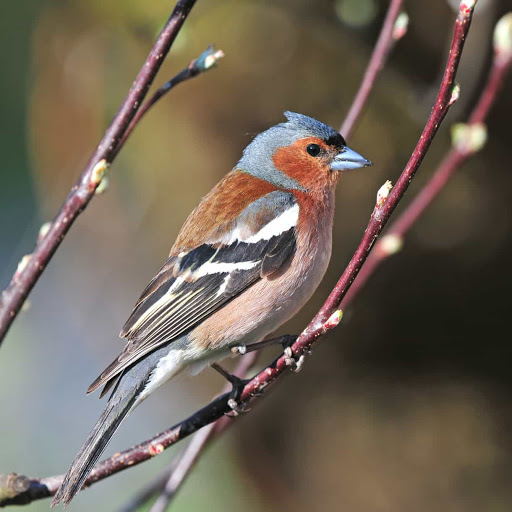
\includegraphics[height=200px]{photo} \caption{Chaff. By Photo © Julia Trafford, \url{http://voice.gardenbird.co.uk/all-about-the-chaffinch/}}\label{fig:chaff-fig}
\end{figure}

\hypertarget{methods}{%
\section{Methods}\label{methods}}

This is the methods!!!

\hypertarget{results}{%
\section{Results}\label{results}}

\hypertarget{discussion}{%
\section{Discussion}\label{discussion}}

\hypertarget{references}{%
\section*{References}\label{references}}
\addcontentsline{toc}{section}{References}

\hypertarget{refs}{}
\leavevmode\hypertarget{ref-rcore}{}%
R Core Team. 2020. \emph{R: A Language and Environment for Statistical Computing}. Vienna, Austria: R Foundation for Statistical Computing. \url{https://www.R-project.org/}.

\leavevmode\hypertarget{ref-tidyverse}{}%
Wickham, Hadley, Mara Averick, Jennifer Bryan, Winston Chang, Lucy D'Agostino McGowan, Romain François, Garrett Grolemund, et al. 2019. ``Welcome to the tidyverse.'' \emph{Journal of Open Source Software} 4 (43): 1686. \url{https://doi.org/10.21105/joss.01686}.

\end{document}
